\begin{que}
	Read about the following plots:
	\begin{enumerate}
		\item Violin Plot
		\item Pareto Chart
		\item Coxcomb Chart
		\item Waterfall Plot
	\end{enumerate}
	Describe the uses of these plots. Take some sample data and generate
	one example plot for each of them.

	\hspace*{\fill} [8 marks]
\end{que}

\begin{tcolorbox}[breakable]
	\begin{sol}
		Here are the descriptions and usages of the given plots along
		with their examples:
		\begin{enumerate}
			\item \textbf{Violin plot:} It's a hybrid of box plot
			      and kernel density plot. A box plot represents
			      data in a linear fashion. It's made of a straight
			      line from lowest value to highest value along
			      with a box from first to third quartiles, marking
			      all the quartiles of the dataset. Here's an
			      example in figure \ref{fig:box}:
			      \begin{figure}[H]
				      \centering
				      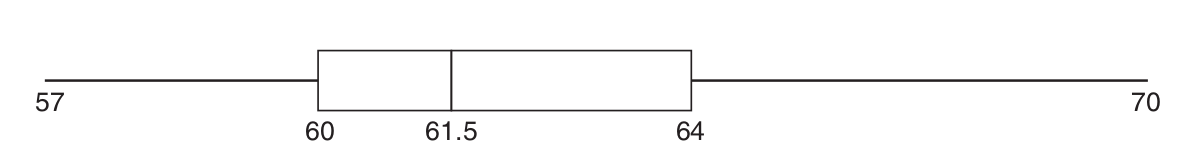
\includegraphics[width=0.5\textwidth]{q7-box_plot}
				      \caption{Box plot}
				      \label{fig:box}
			      \end{figure}
			      A kernel density plot represents the
			      density/frequency of data points. It's similar to
			      a histogram, but smooth. In a violin graph, this
			      is kept vertical, with two mirror images of it
			      reflected along y-axis. This is useful in the
			      sense that we can look into both centrel
			      tendencies of the data (like mean, median etc.)
			      but also how the data is distributed. Both at
			      once. We can visualise the following data which
			      I've taking from (*) containing the average
			      number of hours a person studies given the number
			      of courses taken
			      \begin{figure}[H]
				      \centering
				      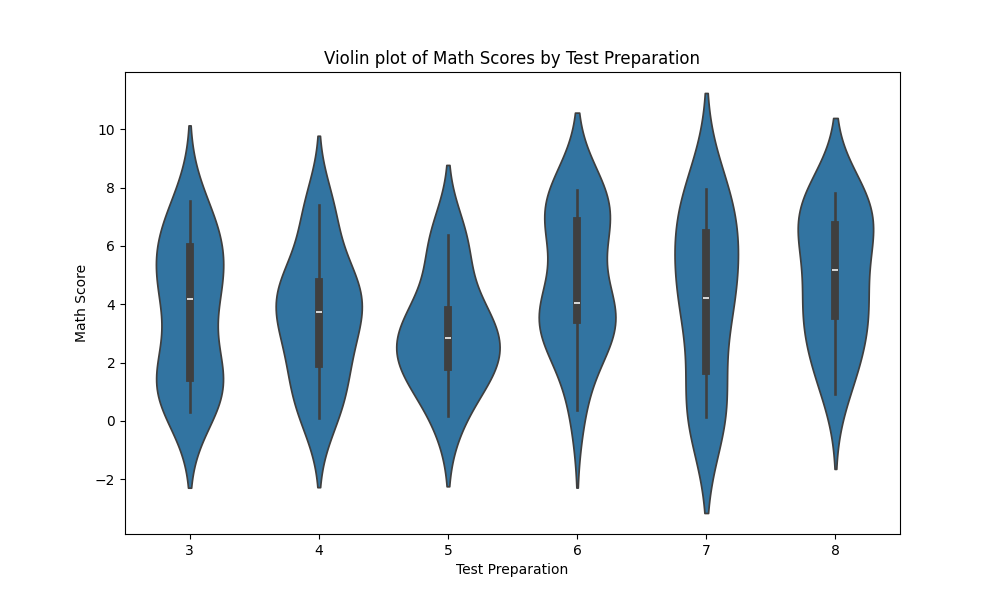
\includegraphics[width=0.7\textwidth]{q7-violin-plot}
				      \caption{Violin Plot}
				      \label{fig:violin}
			      \end{figure}
			      As mentioned before, a violin plot can show both
			      statistical summary along with distribution,
			      which a normal plot can't. Here in figure
			      \ref{fig:violin}, the gray line represents the
			      box plot component of it. And the plot you get by
			      rotating it by $90^\circ$ is the distribution
			      plot.
			\item \textbf{Pareto Chart:}
			      A pareto chart consists of both a bars and a line
			      graph in the same plot. The bar graph represents
			      the individual data like frequency, cost, height,
			      weight of individual values. These values are
			      arranged in decreasing order of the height of
			      corresponding graphs. The line graph represents
			      the cumulative data like frequency, cost, etc.
			      till that point. Since the values decreases, this
			      line graph is concave.
			      \begin{figure}[H]
				      \centering
				      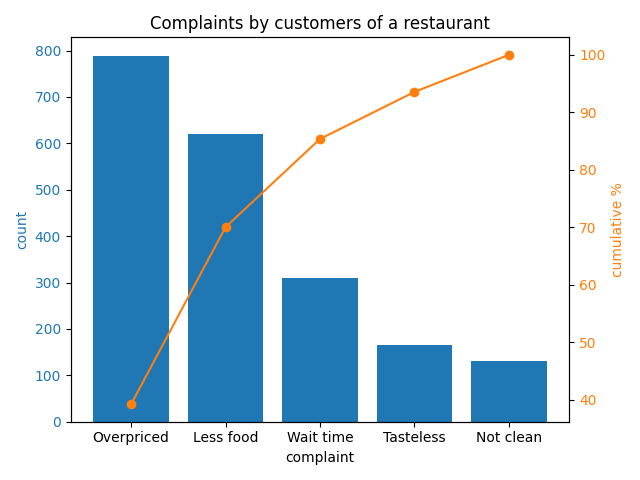
\includegraphics[width=0.7\textwidth]{q7-pareto-plot.png}
				      \caption{Pareto Plot}
				      \label{fig:pareto}
			      \end{figure}
			      An example of a pareto plot is shown where I've
			      collected data of complaints from customers about
			      a given restaurant. It's useful in this case
			      because it is able to show the proportion of the
			      problem particular category is causing as well as
			      the magnitude of the problem.
			\item \textbf{Coxcomb Chart:}
			      A coxcomb chart is similar to a pie chart. It's
			      also known as a polar chart. But unlike a pie
			      chart, here the area of each sector represents the
			      proportion of the problem caused by a particular
			      category of data unlike a pie chart, where the
			      angle represents the proportion.
			      \begin{figure}[H]
				      \centering
				      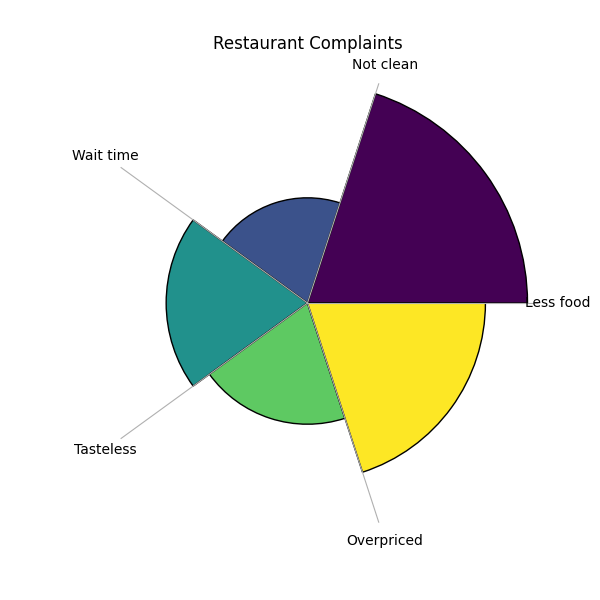
\includegraphics[width=0.5\textwidth]{q7-coxcomb.png}
				      \caption{Coxcomb Plot}
				      \label{fig:coxcomb}
			      \end{figure}
			      Here in figure \ref{fig:coxcomb} I've shown the
			      same data shown before in figure \ref{fig:pareto}
			      in a coxcomb chart. Like a pie chart, a coxcomb
			      chart isn't useful when it comes to to large
			      number of categories of data. It's useful when we
			      have a small number of data which is categorical.
			\item \textbf{Waterfall plot:}
			      A waterfall plot shows how two-dimensional data
			      changes over time, this two-dimensional data is
			      typically a spectra. This results in a 3D graph.
			      But this 3D graph is drawn in a 2D manner, by
			      staggering the curves both accross the screen and
			      vertically. Due to this, the curves in the front
			      ``hide'' the ones behind.
			      \begin{figure}[H]
				      \centering
				      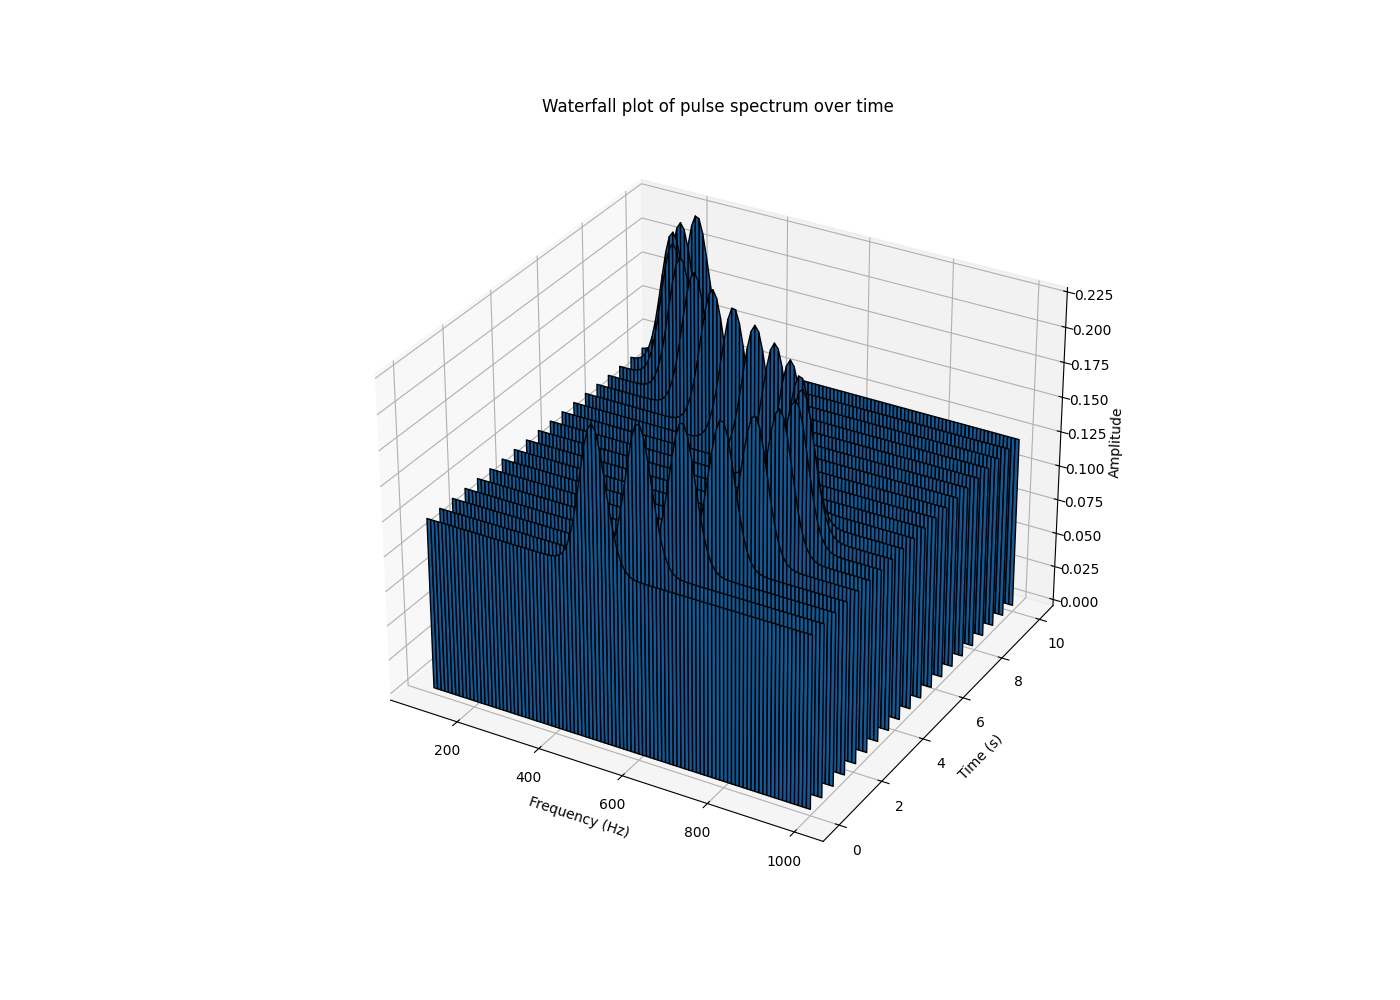
\includegraphics[width=0.9\textwidth]{q7-waterfall.png}
				      \caption{Waterfall Plot}
				      \label{fig:waterfall}
			      \end{figure}
			      This is very useful in
			      studying data which has a spectrum, for example,
			      showing spectrum of a given signal at different
			      intervals of time, spectra at different engine
			      speeds when testing engines etc.
		\end{enumerate}
	\end{sol}
\end{tcolorbox}
